%% LyX 2.0.3 created this file.  For more info, see http://www.lyx.org/.
%% Do not edit unless you really know what you are doing.
\documentclass[a4paper,10pt, times]{article}
\renewcommand{\rmdefault}{cmr}
\renewcommand{\sfdefault}{cmss}
\renewcommand{\ttdefault}{cmtt}
\renewcommand{\familydefault}{\sfdefault}
\usepackage[T1]{fontenc}
\usepackage[utf8]{inputenc}
\usepackage{geometry}
\geometry{verbose,tmargin=2cm,bmargin=2cm,lmargin=3.5cm,rmargin=2cm}

\makeatletter
%%%%%%%%%%%%%%%%%%%%%%%%%%%%%% User specified LaTeX commands.\usepackage[toc]{glossaries}
%\usepackage[estonian]{babel}
\usepackage[russian,estonian,english]{babel}
\usepackage{datetime}


\usepackage{textcomp} % Used for syntax highlighting. 
%\usepackage{listings}
\usepackage{color}
\usepackage{palatino} 
\usepackage{setspace}
\usepackage{needspace} % line skipping

% images
\usepackage{graphicx}
\usepackage{wrapfig}


%\usepackage[printonlyused,withpage]{acronym}


\usepackage[bookmarks=true,
bookmarksnumbered=true,
bookmarksopen=false,
backref=page,
,colorlinks=true]{hyperref}
%\hypersetup{backref=true}
%\usepackage{backref}
%\usepackage{hyperref}
%\usepackage[colorlinks,bookmarks=false]{hyperref}
\usepackage{url}
\usepackage{makeidx}
% bibliography to table of contents
%\usepackage[nottoc,numbib]{tocbibind}

\usepackage{minted}

%\bibliography{references.bib}
% urls in bibliography
%\usepackage{natbib}
%\usepackage{babelbib}

% \usepackage[
%     backend=biber,
%     style=ieee,
%     sortlocale=de_DE,
%     natbib=true,
%     url=false, 
%     doi=true,
%     eprint=false,
%     backref=true
% ]{biblatex}
%\usepackage[style=ieee]{biblatex}
%\addbibresource{references.bib}



\usepackage{float}
\usepackage{tabularx}
% first paragraph indent
%\usepackage{indentfirst}
\usepackage{longtable}



%\input{macros/tables.tex}
%\usepackage{../resource/python}

\usepackage[acronym,footnote,toc]{glossaries}


\makeglossaries

%\newcommand{\estDate}[3]{\begin{otherlanguage}{estonian}\formatdate{#1}{#2}{#3} \end{otherlanguage}}

%\newcommand{\estToday}{\begin{otherlanguage}{estonian}\today \end{otherlanguage}}

%%
%% eestikeelsed kuupa"evad
%%
\def\@kuuaasta{\ifcase\the\month\or
  jaanuar\or veebruar\or mƤrts\or aprill\or mai\or juuni\or
  juuli\or august\or september\or oktoober\or november\or detsember\fi
  \space \number\the\year}

\def\@aasta{\the\year}


\newcommand{\estDate}[3]{%
\begin{otherlanguage}{estonian}
#1.~
\ifcase #2 \relax
\or jaanuar
\or veebruar
\or mƤrts
\or aprill
\or mai
\or juuni
\or juuli
\or august
\or september
\or oktoober
\or november
\or detsemberhttp://staff.ttu.ee/~alahe/ .
\fi
~ #3 .~a.
 \end{otherlanguage}}

\newcommand{\estToday}{\estDate{\the\day}{\the\month}{\the\year}}


%\input{macros/languages.tex}

%  some renamings
\AtBeginDocument{
% estonian language
%\renewcommand{\prefacename}{Sissejuhatus}
%\renewcommand{\abstractname}{KokkuvƵte}
%\renewcommand{\contentsname}{Sisukord}
%\renewcommand{\listfigurename}{Joonised}
%\renewcommand{\listtablename}{Tabelid}
%\renewcommand{\refname}{Viited}
%\renewcommand{\bibname}{Kirjandus}
%\renewcommand{\indexname}{Indeks}
%\renewcommand{\figurename}{Joonis}
%\renewcommand{\tablename}{Tabel}
%\renewcommand{\partname}{Osa}
%\renewcommand{\chaptername}{PeatĆ¼kk}
%\renewcommand{\appendixname}{Lisa}
%\renewcommand{\enclname}{Lisa(d)}
%\renewcommand{\ccname}{Koopia(d)}
%\renewcommand{\headtoname}{Kellele}
%\renewcommand{\pagename}{Lk.}
%\renewcommand{\seename}{vt.}
%\renewcommand{\alsoname}{vt. ka}
%
% russian language
%
%\renewcommand{\prefacename}{Š�Ń€ŠµŠ´ŠøŃ�Š»Š¾Š²ŠøŠµ}
%\renewcommand{\abstractname}{Š�Š½Š½Š¾Ń‚Š°Ń†ŠøѸ}
%\renewcommand{\contentsname}{Š˛Š³Š»Š°Š²Š»ŠµŠ½ŠøŠµ}
%\renewcommand{\listfigurename}{Š�ŠæŠøŃ�Š¾Šŗ Ń€ŠøŃ�Ń�Š½ŠŗŠ¾Š²}
%\renewcommand{\listtablename}{Š�ŠæŠøŃ�Š¾Šŗ Ń‚Š°Š±Š»Šøц}
%\renewcommand{\refname}{Š›ŠøŃ‚ŠµŃ€Š°Ń‚Ń�Ń€Š°}
%\renewcommand{\bibname}{Š›ŠøŃ‚ŠµŃ€Š°Ń‚Ń�Ń€Š°}
%\renewcommand{\indexname}{Š�Ń€ŠµŠ´Š¼ŠµŃ‚Š½Ń‹Š¹ Ń�ŠŗŠ°Š·Š°Ń‚ŠµŠ»Ń�}
%\renewcommand{\figurename}{Š ŠøŃ�.}
%\renewcommand{\tablename}{Š¢Š°Š±Š»ŠøцŠ°}
%\renewcommand{\partname}{Š§Š°Ń�Ń‚Ń�}
%\renewcommand{\chaptername}{Š“Š»Š°Š²Š°}
%\renewcommand{\appendixname}{Š�Ń€ŠøŠ»Š¾Š¶ŠµŠ½ŠøŠµ}
%\renewcommand{\enclname}{Š²ŠŗŠ».}
%\renewcommand{\ccname}{ŠøŃ�Ń….}
%%\renewcommand{\headtoname}{Š²Ń….}
%\renewcommand{\pagename}{�тр.}
%\renewcommand{\seename}{Ń�Š¼.}
%\renewcommand{\alsoname}{Ń�Š¼. Ń‚Š°ŠŗŠ¶Šµ}
%
%
%\renewcommand{\contentsname}{Š˛Š³Š»Š°Š²Š»ŠµŠ½ŠøŠµ}
%
%\frenchspacing
%\setlength{\parskip}{20pt  plus 1pt minus 1pt}
\setlength{\parindent}{1cm}
}

\makeatother

\begin{document}

	%\newglossaryentry{H20}{name=water,description={The equation of wather}}
%\newglossaryentry{FPS}{name=fpsLabel,description={Frame per Second}}
%\newglossaryentry{A}{name=area,description={Area}}

\newacronym{FPS}{FPS}{Frame per Second}
\newacronym{H20}{H20}{The equation of wather}
\newacronym{FPGA}{FPGA}{Field-programmable gate array}
\newacronym{ASIC}{ASIC}{Application-specific integrated circuit}
\newacronym{SOA}{SOA}{Service-oriented architecture}
\newacronym{RPC}{RPC}{Remote procedure call}
\newacronym{IPC}{IPC}{Inter-process communication}
\newacronym{IDL}{IDL}{Interface description language}
\newacronym{JSON}{JSON}{JavaScript Object Notation}
\newacronym{XML}{XML}{Extensible Markup Language}
\newacronym{MCU}{MCU}{Microcontroller}
\newacronym{HMI}{HMI}{Human Machine Interaction}
\newacronym{API}{API}{Application programming interface}

\newacronym{FTP}{FTP}{File Transfer Protocol}

\newacronym{UDDI}{UDDI}{Universal Description, Discovery and Integration}
\newacronym{QoS}{QoS}{Quality of service}

\newacronym{HTTP}{HTTP}{Hypertext Transfer Protocol}
\newacronym{TCP}{TCP}{Transmission Control Protocol}
\newacronym{URI}{URI}{Uniform Resource Identifier}
\newacronym{MIME}{MIME}{Multipurpose Internet Mail Extensions}



\newacronym{SMTP}{SMTP}{Simple Mail Transfer Protocol}
\newacronym{WSDL}{WSDL}{Web Services Description Language}
\newacronym{DPWS}{DPWS}{Devices Profile for Web Services}
\newacronym{SOAP}{SOAP}{Simple Object Access Protocol}
\newacronym{REST}{REST}{Representational state transfer}
\newacronym{CRUD}{CRUD}{Create, read, update and delete}

%java technologies
\newacronym{JVM}{JVM}{Java Virtual Machine}
\newacronym{JMS}{JMS}{Java Message Service}


\newacronym{YAML}{YAML}{YAML Ain't Markup Language}

%HW
\newacronym{DMA}{DMA}{Direct Memory Access}
\newacronym{ISR}{ISR}{Interrupt service routine}
\newacronym{CAN}{CAN}{Controller Area Network}
\newacronym{ARM}{ARM}{Advanced RISC Machine}
\newacronym{USB}{USB}{Universal Serial Bus}
\newacronym{JTAG}{JTAG}{Joint Test Action Group ( IEEE 1149.1 Standard Test Access Port and Boundary-Scan Architecture. )}
\newacronym{SWD}{SWD}{Serial Wire Debug}

\newacronym{UART}{UART}{Universal asynchronous receiver/transmitter}
\newacronym{USART}{USART}{Universal synchronous/asynchronous receiver/transmitter}
\newacronym{RAM}{RAM}{Random Access Memory}
\newacronym{RF}{RF}{Radio frequency}


	
	\begin{titlepage}
	\begin{center}	
		\begin{minipage}[h]{0.01\linewidth}
			\begin{flushleft}	
				
\includegraphics[scale=0.2]{../images/template/ttu_logo_2.jpg}
			\end{flushleft}		
		\end{minipage}
		\begin{minipage}[h]{0.98\linewidth}
			\begin{center}
				
				\textbf{TALLINN UNIVERSITY OF TECHNOLOGY}\\			
				Faculty of Information Technology \\			
				\textit{Department of Computer Engineering} \\			
		
			\end{center}
		\end{minipage}
	\end{center}
	\vspace{3cm}
	
	\begin{center}
		Denis Konstantinov \footnotesize \textsf{111615 IASM}
	\end{center}
	
	\vspace{5em}
	
	\begin{center} 
		\Large {Embedded service oriented microcontroller architecture.}\\
		\vspace{1em}
		\small {Extensible client-server communication architecture for small
		devices}\\
	\end{center}
	
	\vspace{2em}
	
	\begin{center}		
		\textsf{Master thesis}
	\end{center}
	
	\vspace{2cm}
	
	% Author and supervisor	
	\begin{flushright}		
			%\large \emph{Esitatud:} & \quad \estDate{23}{10}{2008}  \\		
			%\large \emph{Submitted:} & \quad {\the\day}.{\the\month}.{\the\year}\\
			
			\emph{Supervisor:} \quad Peeter Elervee \\
			\small{Associate Professor at the Department of Computer Engineering / Ph.D., Dipl.Eng.}		
	\end{flushright}
	
	\vspace{\fill}
	\begin{center} 
		Tallinn \the\year
	\end{center}	
\end{titlepage}
		
	\clearpage\vspace*{\fill}

\section*{Author's Declaration} 


This work is composed by myself independently. All other authors' works, essential
states from literary sources and facts from other origins, which were used during the
composition of this work, are referenced.

\vspace{7em}
Signature of candidate: \hspace{10em}Date:

\vspace{\fill}
\clearpage



	
	\printglossaries
	
	\clearpage\vspace*{\fill}
\section*{Annotation}
Current work introduces conceptual approaches for implementing an extensible
service oriented client-server application on a small microcontroller.
This is a general-purpose transport and hardware independent embedded server
that uses remote procedure calls as primary communication protocol.
This server looks like remote service that could provide defined functions to
the client.

This paper has a research about available service oriented architecture technologies and reviews them in the context of embedded resource constrained hardware systems.

There is also an implementation of a small embedded service and corresponding client.
Service part is implemented on STM32F1 family ARM Cortex-M3 microcontroller and runs FreeRTOS operating system.
It controls a remote object, that is connected over serial line and uses some closed protocol. 
This server device is a bridge between client and controlled remote object. 
It translates all communication between them and can be used to integrate proprietary or legacy system into existing environment. 

Client part is realized as Java RPC stub library  and Android demo application, which is capable to execute some functions on the remote object.
An example of controlled device here is the coffee machine, which can prepare a cup of coffee for remote client.

Client and server are communicating using lightweight JSON-RPC protocol over Bluetooth wireless communication line.
Some few RPC call functions are implemented to show the capabilities of such client-server architecture.

This work contains several possibilities how to organize communication between different embedded systems.

\vspace{\fill}
\clearpage
	\clearpage\vspace*{\fill}
\section*{Annotatsioon}
Käesolevas töös kirjeldatakse kuidas rakendada teenusorienteritud klient server arhitektuuri sardmikrokontrolleril.
See on üldotstarbeline transport ja riistvara sõltumatu rakendusserver,
mis kasutab kaugprotseduuri väljakutseid kommunikatsiooni pidamiseks.
Mikrokontrolleris jooksev programm näeb välja nagu serveri teenus,
mis pakkub kasutajale ettenähtud funktsionaalsust.

Antud töö eesmärk on teha uuring teenus orienteeritud arhitektuuride ja tehnoloogiate kohta 
ning analüsida nende kasutamist piiratud ressursidega sardsüsteemide realiseerimises.

All on toodud realiseeritud teenusorienteritud sardsüsteemi kirjeldus ja sellele vastav kliendi rakendus.

Serveri pool on tehtud STM32F1 pere ARM Cortex-M3 mikrokontrolleri baasil, kus jookseb FreeRTOS reaalaja operatsioonisüsteem.
Kliendi rakendus on mobiilsel platformil kasutatav programm, mis kasutab Javas kirjutatud teegi kaugprotseduuride väljakutsemiseks.

Klindi ja serveri vaheline kommunikatsioon toimub labi traadita Bluetooth kanali kasutades JSON-RPC protokolli.
Süsteemis on tehtud mõned funktsioonid, selleks et näidata antud klient-serveri arhitektuurilisi omadusi.


\vspace{\fill}
\clearpage
	
	\pdfbookmark{\contentsname}{contents}
	\tableofcontents
	
	
	\newpage
\section{Introduction}

%\subsection{Contributions}



% This is a test of acronyms  \gls{ASIC} \\
% 
% This is a test of code listings
% \begin{listing}[H]
% 	\inputminted[linenos=true,
% 	fistline=32,
% 	firstnumber=32,
% 	lastline=60]{java}{../source/CoffeeMachineViaBlueTooth.java}
% 	\caption{Example of a listing.}
% 	\label{lst:example}
% \end{listing}


% At first here will be lots of words about this cruel world and how it was
% changed in resent years.
% 
% Speech about reusable components.
% 
% Speech about small mobile devices that are everywhere.
% 
% 
% 
% Communication.
% 
% Interaction.





Computers are very essential in our life. Computer is an electronic device that
is used in almost every field. It is very accurate, fast and can accomplish
many tasks easily. In early days computers were only used by the government
and army to solve different high computational tasks. After invention of
low-cost microprocessors, computers became available to every person. Nowadays  
there are billions of personal computers and they are almost at every home.

Present day computers may be divided into two groups: very big and very small systems. In one group are mainly servers and
server farms, and in the other are mainly embedded systems. 
The gap between these groups becomes more wider, because of the availability of new small and low-power devices, which computational power raises constantly.
Lot of people prefer now to buy a tiny laptop instead of traditional workstations with a monitor and computer case under the table.
There is also a more smaller group of devices, that are implemented for a particular purpose - embedded computers.  
Every home has several examples of embedded computers.
Any appliance that has a digital clock, for instance, has a small embedded microcontroller that performs no other task than to display the clock.
Modern cars have embedded computers onboard that control such things as ignition timing and anti-lock brakes using input from a number of different sensors.


Today, there is very little or no communication between embedded devices and large servers in the web.
The problem is not only in the communication infrastructure, because the current communication technologies are able to provide different wired and/or wireless connections.
The problem is how we design and implement embedded systems. While we
try to keep big systems as open as possible (since it is their primary role), we tend to seclude and isolate embedded systems without providing easy ways to add a
custom interface to them. Embedded systems are still mainly seen as vendor-specific and task-oriented products, and not as components that can be easily manipulated and reused.

If all classes of devices could speak the same language, they could 
talk directly to each other in ways natural to the application without artificial technical barriers. This would allow easily 
creating seamless applications that aggregate the capabilities of all 
the electronics. The interoperation adds value to all the devices.

This idea comes from conception of Internet of Things (IoT). The Internet of
Things is the network of physical objects that can communicate to each other
using Internet and embedded technologies. This
connections compose an complex system where each member can send information
about its state and acquire data about other parties without any intervention of
human being.
For example sensors at your home could communicate to heater
and ventilation system and control temperature and humidity or your alarm can
tell all other devices that you are going to wake up soon. 
This technologies could help to track and count everything and improve the
quality of our lives by removing the unnecessary waste and additional cost.


The Internet of Things is quite popular topic of research nowadays. It possibly
can change the world like the Internet did. Many companies and universities are
trying to find and invent reasonable technologies for implementing this approach.

One of the methods how this communication can be performed is the concept of
remote services and service oriented architecture (SOA).
World Wide Web Consortium (W3C) defines a "Web service" as: 
\begin{quote}
A Web service is a software system designed to support interoperable machine-to-machine interaction over a network.
It has an interface described in a machine-processable format (specifically
\gls{WSDL}).
Other systems interact with the Web service in a manner prescribed by its
description using \gls{SOAP}-messages, typically conveyed using \gls{HTTP} with
an \gls{XML} serialization in conjunction with other Web-related standards.
\end{quote}

Services are unassociated, loosely coupled units of functionality.
Not only large server system are capable of providing this functionality.
Services can also be applicable in the resource-constrained embedded devices.

This work would introduce the concepts how \gls{SOA} can be in the  context  of 
embedded  systems.
This contains some research of already available technologies for
machine-to-machine communications and the implementation of small system
prototype, which contains two connected devices and uses service approach.

\subsection{Impact}
The impact of the research in this thesis has been started during the accomplishment of internship at the university. 
I was worked for some company and my task was to develop \gls{HMI} interface to some embedded system.
We were using wireless communication between the control unit and the machine it was controlling.
Control unit was a smartphone that was sending commands through Bluetooth protocol.
On the other side there was a coffee machine that was receiving and executing that commands.

At the same time i was studying how large enterprise systems communicate to each other.
I was reading about web services and related technologies.
Then was born an idea that there could also be a "small" device network, where
devices communicate to each other.

This was a research project and developed prototype could potentially become a real product.
In that case it needs to be connected to existing infrastructure.
Coffee machine could provide different remote services: remote coffee product
ordering, coffee machine maintenance and acquisition of statistical data, remote
payment.
This could look like traditional coffee automatic machines at the streets that
accept cash, but with a remote wireless control.

I stated to mine the information about different control possibilities.
This is how this research became a topic of my master thesis. 

\subsection{The task}

The purpose of this work is to create a prototype system which has remote
service capabilities and make a research of available machine-to-machine
communication possibilities.
This should be an universal and platform independent architecture, which can be easily ported to any suitable hardware and connected
into existing infrastructure. 

Already existing hardware are two STM32f103xx family microcontrollers which have
20 and 64 Kbytes of \gls{RAM}, 128 and 512 Kbytes of flash memory. They are also
equipped with \gls{UART} communication and whole communication need to work using
serial line. Remote server with service capabilities should work on that
hardware. General requirement for the hardware is low-cost microcontroller with
some connectivity, that does not make the  already existing system more
expensive and in the same time fulfil all required functionality.

Embedded server will be connected to a target device, which is actually a coffee
machine, and handle requests from clients by executing various functions on
target device.
Server should provide a functional interface to the client and know about
available functions inside coffee machine. That interface need to be verbose and
easy to connect. 

Client will be executed on mobile phone and will communicate with remote server
using Bluetooth wireless technology. It might be any mobile platform, but
the organization decided to try Google Android smartphones first. 
Android device need to have running program with a graphical user interface,
which is able connect to remote service and accomplish functional needs.

We need to be able to switch existing client hardware architecture and the to
choose various clients for this embedded service. It might be an Android mobile
application, regular desktop computer program or even web application.
It is good to have one common client code that will be used in these different
environments. We should write a client library, which have bindings to the
remote service and handles all the communication. It should provide a
convenient interface to a library client.

Coffee machine application is only the example of such architecture.
We need a real world problem and device to show all capabilities of such system.
Controlled device and the client application could vary. It might be a
remote light control at home or any data acquisition and control system at the
production plant. During this work such universal and extensible system will be
built.

To summarize and make our goal more complete we should make a list and follow
it:
\begin{enumerate}
  \item Make a research about available device-to-device connectivity
  techniques, software standards and communication protocols. Get current state
  of the art and find a suitable technology for the existing environment
  \item Get familiar with already existing hardware tools, setup programming
  environment and write some sample programs to test the capabilities.
  \item Implement service oriented architecture on a microcontroller hardware.
  \item Write some test functionality to prove chosen approach.
  \item Implement a client library software module.
  \item Create a test application that will use this client module inside the
  system and show how it can be applied. 
\end{enumerate}

This work will cover every step in this list and author will try to complete it. 

\subsection{Outline}

The first section will introduce available technologies of implementing
machine-to-machine communications. 
The main research is about the Internet technologies and concept of remote web services, this is because the Internet
is already an interconnected network with lots of machines are doing distributed
computing and interacting with each other. 
Lots of problems are already solved there and there are available different technologies and tools.
Although, all these already implemented features are not limited  only with the
Internet and related technologies like \gls{TCP}/IP and HTTP. 
Some essential features may be extracted from there and ported to resource-constrained devices.
The first section will also cover some connection and interaction possibilities that embedded systems have.

\nameref{sec:implementation} section covers embedded system prototype, that uses
concepts from different machine-to-machine communication technologies. It
contains description of architecture and software and hardware was used. 
Embedded service was implemented on a microcontroller device. 
\nameref{sec:embedded_service_impl} section covers the hardware and software parts of the system.

\nameref{sec:java_library} section describes the details of Java client stub library.
There is also implementation of a demo client application  in the section next to it. 
This is the last section here.



	\newpage
\section{Preliminaries}

Internet technology is the environment in which billions of people and trillions of
devices are interconnected in various ways.
As part of this evolution, Internet becomes the basic carrier
for interconnecting electronic devices – used in industrial
automation, automotive electronics, telecommunications
equipment, building controls, home automation, medical
instrumentation, etc. – mostly in the same way as the Internet came
to the desktops before. More and more devices getting connected to World Wide
Web. Variety of factors have incluenced  this evolutions \cite{4221180}:
\begin{itemize}
\item The availability of affordable, high-performance, low-power
electronic components for the consumer devices. Improved technology can assist
building  advanced functionality into embedded devices and enabling new ways of
coupling between them.
\item Even low cost embedded devices have some wired or wireless interface to local area
networks of the Ethernet type. TCP/IP family protocols are becoming the standard
vehicle for exchanging information between networked devices.
\item The emergence of platform independent data interchange mechanisms based on
Extensible Markup Language (XML) data formatting gives lots of opportunities for developing high-level data interchange and
communication standards at the device level.
\item The paradigm of Web Services  helps to connect various
independent applications using lightweight communications. Clients that are
connected to the service and the service itself may be written using different
programming languages and be executed on different platforms.
\item Presence of Internet allows existing of small embedded controllers and
large production servers in the same network, with a possibility to change
information.
\end{itemize}


The integration of different classes of devices, which employ different
networking technologies, is still an open research area. One of the possible
solutions is the use of SOA software architecture design pattern.



\subsection{Service oriented architecture}
\begin{quote}
Service-oriented computing is a computing paradigm that uses services as basic building blocks for
application development.
\cite {lws_milanovic.pdf}
\end{quote} 

The purpose of \gls{SOA} is to allow easy cooperation of a large number of
computers that are connected over a network.
Every computer can run one or more services, each of them implements one
separate action. This may be a simple business task. Clients can make calls
and receive required data or post some event messages.

Services are self-describing and open components. There is a service interface,
that is based on the exchange of messages and documents using standart formats.
Interface internals ( operating system, hardware platform, programming language)
are hidden from client. Client uses only a service specification scheme, also
called contract. Consumers can get required piece of funcionality by mapping problem
solution steps to a service calls. This scheme provides quick access and easy integration of software components.


Service architecture have been successfully adopted in
business environments. Different information systems, that were created inside
companies for automation of business processes,  are now turned into services
which may easily interact with each other. For example, Estonian goverment uses
services to transmit data between information systems of different departments.
There are also some free services available. Some Internet search companies like
Google, Bing, Yandex provide lots of alternatives how to retrieve data without
using regular browser( search , geolocation and maps,  spell check \gls{API}s )

There are available many techologies which can be used to implement
\gls{SOA}~\cite{wikipedia:SOA}:
\begin{itemize}
  \item Web Services
  \item{SOAP} Simple Object Access Protocol, is a protocol specification for exchanging structured information in the implementation of Web Services in computer networks.
  \item{RPC} Remote procedure call is an inter-process communication that allows
  a computer program to cause a subroutine or procedure to execute in another address space (commonly on another computer on a shared network) without the programmer explicitly coding the details for this remote interaction. 
  \item{REST} Representational state transfer is a style of software architecture for distributed systems such as the World Wide Web. REST has emerged as a predominant web API design model.
  \item{DCOM} Distributed Component Object Model is a proprietary Microsoft technology for communication among software components distributed across networked computers. 
  \item{CORBA}  Common Object Request Broker Architecture enables separate pieces of software written in different
    languages and running on different computers to work with each other like a single application or set of services. Web services
  \item{DDS} Data Distribution Service for Real-Time Systems (DDS) is an Object
  Management Group (OMG) machine-to-machine middleware standard that aims to
  enable scalable, real-time, dependable, high performance and interoperable data exchanges between publishers and subscribers. 
  \item{Java RMI} Java Remote Method Invocation is a Java API that performs the
  object-oriented equivalent of remote procedure calls (RPC), with support for direct transfer of serialized Java objects and distributed garbage collection.
  \item{Jini}  also called Apache River, is a network architecture for the construction of distributed systems in the form of modular co-operating services.
  \item{WCF} The Windows Communication Foundation (or WCF), previously known as
  "Indigo", is a runtime and a set of APIs (application programming interface)
  in the .NET Framework for building connected, service-oriented applications.
  \item{Apache Thrift} is used as a remote procedure call (RPC) framework and
  was developed at Facebook for "scalable cross-language services development".
  \item \ldots
\end{itemize}

This list can be continued. Most of these technologies are inspired by idea
of \gls{RPC}. An \gls{RPC} is initiated by the client, which sends a request
message to a known remote server to execute a specified procedure with specified
parameters. The remote server sends a response to the client, and the application continues its process.

Web Services are the most popular technology for implementing
service-oriented software nowadays. Next section will focus on this framework
and on the main features that any \gls{SOA} implementation should have.
 
\subsection{Web Services architecture}
\subsubsection{Web Services Model}
The Web Services architecture is based on the interactions between three
roles \cite{Kreger2001-WSC}:
service provider, service registry and service requestor. 
This integration has of three operations: publish, find and
bind. The service provider has an implementation of service. Provider defines a
service description and publishes it to a service requestor or service registry.
The service requestor uses a find operation to retrieve the service
description locally or from the service registry and uses the service description to bind with the
service provider and invoke or interact with the Web service implementation.
\autoref{fig:ws_model} illustrates these service roles and their operations.


\begin{center}
 \begin{figure}[H]
	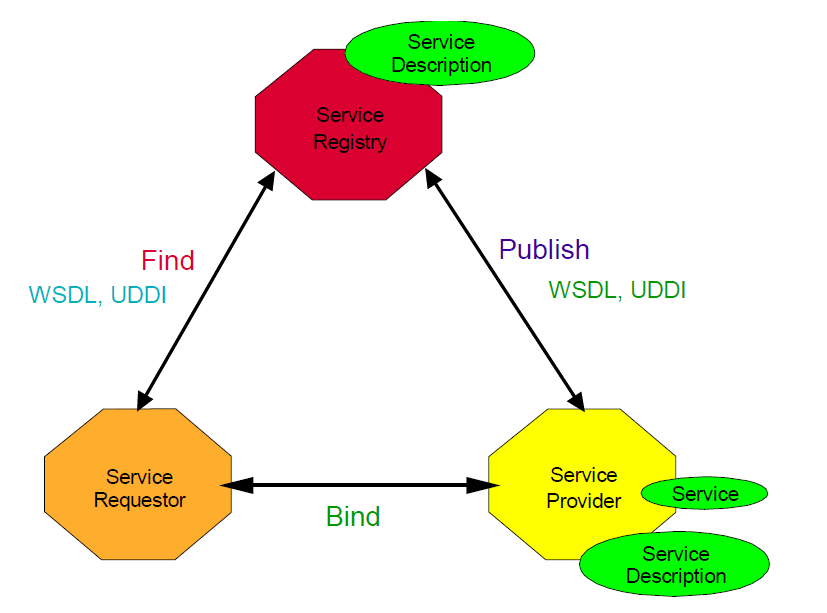
\includegraphics[width=\textwidth]{../images/preliminaries/ws_model.png}
	\caption{Web Services roles, operations and artifacts \cite{Kreger2001-WSC}}
	\label{fig:ws_model}
 \end{figure}
\end{center}

Service registry is a place where service providers can publish
descriptions of their services. Service requestors can find service descriptions
and get binding information from them. Binding can be static and dynamic.
Registry is needed more for dynamic binding where client can get service info at
the runtime, extract necessary functional methods and execute them on the
server. During static binding service description may be directly delivered to
the client at the development phase, for example using usual file, \gls{FTP}
server, Web site, email or any other file transfer protocol.
There are also available special protocols, named Service discovery protocols
(SDP), that allow automatic detection of devices and services on a network. One
of them is the \gls{UDDI} protocol, which is also was mentioned on
\autoref{fig:ws_model}. \gls{UDDI} is shortly described in
\nameref{sec:ws_protocol_stack} section.

\paragraph{\textbf{Artifacts of a Web Service}}
\newline
Web service consists of two parts~\cite{Kreger2001-WSC}:
\begin{itemize} 
\item \label{itm:service_description_artifact} 
\textbf{Service Description}~~~The
service description contains the details of the interface and implementation of the service. This includes its data types, operations, binding
information and network location. There could also be a categorization and
other metadata about service discovery and utilization. It may contain some
Quality of service (QoS) requirements. 

 \item \textbf{Service}
 ~~~This is the implementation of a service - a software module deployed on network accessible platforms provided by the service provider.
 Service may also be a client of other services. Implementation details
 are encapsulated inside a service, and client does not know the details how
 server processes his request.
\end{itemize}



\subsubsection{Web Services Protocol Stack}
\label{sec:ws_protocol_stack}

WS architecture uses many layered and interrelated technologies.
\autoref{fig:ws_protocol_stack} provides one illustration of some of these technology families.

\begin{center}
 \begin{figure}[h]
	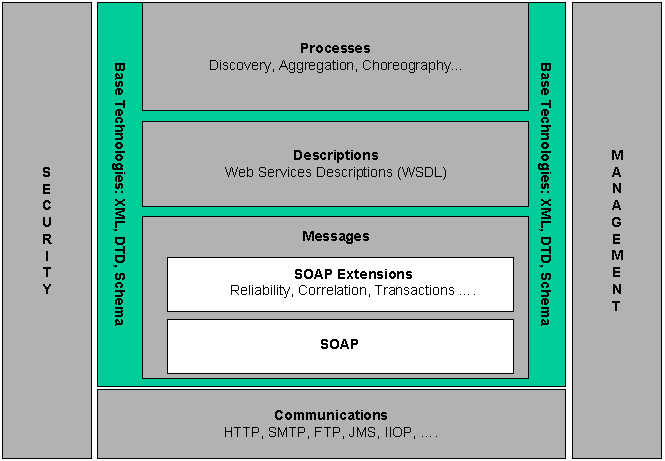
\includegraphics[width=\textwidth]{../images/preliminaries/ws_protocol_stack.png}
	\caption{Web Services Architecture Stack \cite{ws_arch} }
	\label{fig:ws_protocol_stack}
 \end{figure}
\end{center}

We can describe these different layers as follows:
\begin{itemize}
  \item \textbf{Communications} - This layer represents a transport between
  communication parties( service provider, client, service registry). This layer
  can be any network protocol like: \gls{HTTP}, \gls{FTP}, \gls{SMTP} or any
  other suitable transport protocol. If Web service is used in the Internet, the
  transport protocol in most cases will be \gls{HTTP}. In internal networks there is the opportunity to agree upon the use of alternative
network technologies.

\item \textbf{Messages} - In order to communicate with a service, client should
send a message. Messages are \gls{XML} documents with different structure.
\gls{SOAP} protocol defines how these messages should be structured.
\gls{SOAP} is implementation independent and may be composed using any
programming language. Protocol specification and message descriptions can be
found in document SOAP Version 1.2 Part 1: Messaging Framework (Second
Edition)\cite{soap_protocol_spec}.

\item \textbf{Descriptions} - This layer contains the definition of service
interface (see also \autoref{itm:service_description_artifact}). Web Services
use \gls{WSDL} language for describing the functionality offered by a service.
\gls{WSDL} file is the contract of service, which contains information about how
the service can be called, what parameters it expects, and what data structures it returns.
It is similar to method signatures in different programming languages.

\item \textbf{Processes} - This part contains specifications and protocols
about how service could be published and discovered. Web services are meaningful
only if potential users may find information sufficient to permit their execution.
Service as a software module has its own lifecycle, it needs to be deployed and deleted somehow.
Traditional Web Services use \gls{UDDI}  mechanism to register and locate web
service applications. \gls{UDDI} was originally proposed as a core Web service
standard.
  
  
 
\end{itemize}

\subsubsection{Basic Service Description and Service Contract}
\label{sec:ws_service_contract}
Basic Service Description

\subsection{SOA and Embedded Systems}


\subsubsection{Authentication and Authorization in embedded systems}
\paragraph{Need of security}
Authorization is the process of granting or denying access to a network resource.
Most computer security systems are based on a two-step process.
The first stage is authentication, which ensures that a user is who he or she claims to be.
The second stage is authorization, which allows the user access to various resources based on the user's identity. 

Users are essential part of every system. System should be designed with
a requirement, that there will be at least one user. System without any purpose
does not make sense. Usually information systems have lots of users with
different roles. There should be an system administrator - the most authorized individual
in the system, managers and normal users. System should distinct them all
somehow. 

Another requirement is system and information security. System may contain
sensitive data, that should not be available to general users. In case of remote
services there are some services that are not open. These services or some
of their parts are require some identity to pass through. 

Let's take a usual website as example. Common website has at least three
different user roles:
user or guest, content publisher and system administrator. Last two roles may be
joined together, but in general content publishers do not do system maintenance, they
just work with content of webpages. There may be more different roles, but these
are the main ones. Imagine you open a web page and you see the content. You
follow the links and surf the web site. If you want to change something, for
example you do not like the design or some words on web page were misspelled,
you need to find special place where you can input your \textbf{credentials} and
get into the system. This will happen only if you have proper
\textbf{permission} to do that. When you get inside you are still not able to do
anything due to lack of privileges. For example you cannot turn of the
webserver or disable the your website. There may be lots of different roles and
responsibilities in the system and each role has limited access to system
resources.

Embedded device as a service may be similar to system example above. Device may
have some limited use cases, that are not available to not authorized service
clients. This may be internal information retrieving, some  device
manipulation functions (turn on/off something, delete/remove something from the
system, change of system preferences). Some device functionality may be
available only for limited people, for example system owner. The real life example of such system is the wireless
router. Router clients are other computers, they can send and receive network
packets. Router uses wireless security protocols, which permit unauthorized
access. Even if you are connected to a secure access point, you are not able to
change system settings. You should have admin permission (password) to manage
the system. This kind of system, like many embedded systems, is made for one
purpose. Router purpose is to provide access for the network. You also can
remember lots of similar systems, that use authorized access. Nowadays it is not new to get
remotely into some device and to change internals, but embedded system
integrations are still not so common. Imagine near future, you are sitting at
work and thinking to go home. After a long day you became really hungry. You
take your smartphone and connect to your remote wireless fridge service at home. You type
your password and get list of all food in your fridge. Now you know what you
need to buy and the real candidates to be throwed to the rubbish bin. You adjust
power in some fridge area and your beer will be very cold when you get home. Is
it just a dream? Is it really hard to realize using present time technologies?


The main problem here is the security. Wired embedded network protocols are
mostly not designed with security in mind. These networks were isolated from the
Internet in the past. They could only be attacked using direct physical access
to the network. Nowadays Internet and wireless networks are popular. Lots of
communication between different systems goes through the wireless channel. Radio link is also available to your neighbour behind the wall. Generally, you do not want to broadcast what is in your fridge or to give ability to connect to your air conditioning service. Therefore you need to use some authentication scheme for
your service.

\paragraph{Authentication protocols}

Authentication is any process by which you verify that someone is who they claim
they are. (https://httpd.apache.org/docs/2.2/howto/auth.html)

Humanity has already invented a lot of different authentication techniques. 

The ways in which someone may be authenticated fall into three
categories: (http://en.wikipedia.org/wiki/Authentication)
\begin{itemize}
  \item the ownership factors: Something the user has (e.g., wrist band, ID
  card, security token, software token, phone, or cell phone)
  \item the knowledge factors: Something the user knows (e.g., a password, pass
  phrase, or personal identification number (PIN), challenge response (the user must answer a question), pattern)
  \item the inherence factors: Something the user is or does (e.g., fingerprint,
  retinal pattern, DNA sequence (there are assorted definitions of what is sufficient), signature, face, voice, unique bio-electric signals, or other biometric identifier).
\end{itemize}

Authentication may be one way (only client is checked for validity) and two way
( both client and server check each other). Some systems  may requre to use
different security factors together: you say password, provide ID card and show
you fingerprint There are also available many standard authentication protocols.
If you start searching you will probably find similar list:
\begin{itemize}
  \item Transport Layer Security (TLS)
  \item Extensible Authentication Protocol (EAP)
  \item Password authentication protocol (PAP)
  \item Challenge-Handshake Authentication Protocol (CHAP)
  \item Password-authenticated key agreement
  \item Remote Authentication Dial In User Service (RADIUS)
  \item Kerberos
  \item Lightweight Extensible Authentication Protocol (LEAP)  
\end{itemize}

Choosing suitable protocol is not trivial problem. There is no any case general
protocol.  Most of them are designed to interconnect big computers inside a
network. Mostly they operate on transport and application level and use TCP/IP
protocol stack.

All these protocols could be devided into these groups:
\begin{itemize}
  \item Protocols that transmit the secret over the network. (For example
  Password authentication protocol). These protocols are not secure.
  \item Protocols that not send secrets and provide authentification through
  sending messages. (CHAP and Password-authenticated key agreement).
  \item Protocols that require a trusted third party.  
\end{itemize}

Protocols of first type have been deprecated because of security reasons. They
send sensitive data over the network and everyone else between two nodes can
catch this data.

Second group of protocols was invented because the first group was unable to
provide proper level of security. Link between client and server (two parties)
does not contain pure information about the secret. Parties use cryptography and
send encrypted messages to each other. Finally they authenticate each other when there is enough information gathered to validate the authority.

Last group uses trusted third party authority to check each other. There is
assumption that all three parties should have connection between each other. Embedded device during
client authentification needs to connect some server and ask for a secret. Third
party should always have a high authority, two other parties should trust him.
This scheme should be used in case of high security requirements.



Choosing of right authentication protocol in general should depend on application.
Sometimes, there will be enough just to send plain text passwords over the
network.
Engineer should analyze all hazards during system design process.

Lifecycle of an embedded system is more longer than livecycle of average personal computer. Application specific controller  may run for decades and it will be still functional.
Choosed security algorithm may be not secure enough after some years. Some vulnerabilities can be discovered during that period. 
Computational power of modern processors raises every year and  secure encryption may be cracked during some seconds in the future.
There is no 100\% secure system, everything can be breaked. 

Your system security should have such encryption, that provides proper security
level to your application data and can not be cracked quickly.
How quick it is depends on your data and security requirements of your data.

Another aspect is the complexity of cryptography algorithms. Embedded devices
are usually small low power devices with limited computation abilities. Not
every algorithm suits well. It should be quick and resource friendly , and in
same time it should be secure.

Nowadays, the last versions of the Wifi and Wimax standards include the use of
Extensible Authentication Protocol (EAP) declined in different versions
(LEAP - EAP using a Radius Server -, EAP-TTLS, etc...). In practice, EAP is interesting for workstations or desktop computers but does not fit the needed security of particular systems such as handheld devices, short-range communication sys- tems or even domestic Wireless LAN devices. The reason being that many versions of EAP use certificates,
public key encryption or exhaustive exchanges of information, that are not viable for lightweight wireless
devices.[A new generic 3-step protocol for authentication and key
agreement in embedded systems]

Protocol should small in code size. You should not to place a
separate controller, which deals with communication,  into your system.
Everything is needed to be inside one small and cheap device. Business requires
as low price as possible, because only that it could give you any money.


Embedded networking has constraints that developer should keep in mind
while developing a system.

% There are already available small realizations of TCP/IP stack that could be run
% [ssylka na doktorskuju Programming
% Memory-Constrained
% Networked Embedded Systems] on small 8-bit microcontrollers, but they have only
% limited protocol stack and security protocols need to be provided separately.
% 
% There are  

\paragraph{Embedded Network Constraints} [A Flexible Approach to Embedded Network
Multicast Authentication]
Embedded networks usually consist of a number of Electronic Control
Units (ECUs). Each ECU performs a set of functions in the system. These ECUs are
connnected to a network, and communicate using a protocol such as CAN,
FlexRay, or Time-Triggered Protocol (TTP). These protocols are among the most
capable of those currently in use in wired embedded system networks. Many other protocols are even
less capable, but have generally similar requirements and constraints:

\begin{itemize}
  \item{Multicast Communications} - All messages sent on a
distributed embedded network are inherently multicast,
because all nodes within the embedded system need to
coordinate their actions. Once a sender has transmitted a
packet, all other nodes connected to the network receive the
message. (In CAN, hardware performs message filtering at the
receiver based on content.) Each packet includes the sender's
identity, but does not include explicit destination information. The configuration of the network is
usually fixed at design time, and changes a littel or  does not change at all.
\item{Resource Limited Nodes} - 
Processing and storage capabilities
of nodes are often limited due to cost considerations at design
time. Controllers, that are used usually have no more than 32 kilobytes of RAM
and 512 kilobytes of Flash memory. Their operating frequency is no more than 100
MHz. Authentication mechanisms which require large amounts of
processing power or storage in RAM may not be feasible.
\item{Small Packet Sizes} - Packet sizes are very small in embedded
network protocols when compared to those in enterprise
networks. The bandwidth is very limited. Network synchronization and packet
integrity checks should be added to this. For example data rates are limited to
1 Mbit/sec for CAN and 10 Mbit/sec for TTP and FlexRay. Devices cannot store
large packets in memory during processing, as it was mentioned in previous
requirement. Authentication should have minimal bandwidth overhead.
\item{Tolerance to Packet Loss} - Embedded systems often work in a
very noisy environment. Data may corrupt during transmission. Authentication
schemes must be tolerant to packet loss.
\item{Real-Time Deadlines} - In real-time safety-critical systems, delays are
not tolerated. Processes should be completed within specified deadlines.
Authentication of nodes must occur within a known period of time. There should
not be unspecified delays.
\end{itemize}


\paragraph{Challenge-Handshake Authentication}

In this work i decided to use Challenge-Handshake Authentication Protocol
[http://tools.ietf.org/html/rfc1994].

CHAP is an authentication scheme used by Point to Point Protocol (PPP) servers to validate the identity of remote clients. 
CHAP periodically verifies the identity of the client by using a three-way handshake. 
This happens at the time of establishing the initial link (Link control protocol), and may happen again at any time afterwards.
The verification is based on a shared secret (such as the client user's
password).
\begin{enumerate}
  \item After the completion of the link establishment phase, the authenticator
  sends a "challenge" message to the peer.
  \item The peer responds with a value calculated using a one-way hash function
  on the challenge and the secret combined.
  \item The authenticator checks the response against its own calculation of the
  expected hash value. If the values match, the authenticator acknowledges the authentication; otherwise it should terminate the connection.
  \item At random intervals the authenticator sends a new challenge to the peer
  and repeats steps 1 through 3.
\end{enumerate}

The secret is not sent over the link.
Although the authentication is only one-way, you can negotiate CHAP in both directions, 
with the help of the same secret set for mutual authentication.

This protocol is described in the document [http://tools.ietf.org/html/rfc1994].
Document specifies main protocol consepts and packet formats.

There are some procol extensions like MS-CHAP and CHAP is used
as a part of other protocols like EAP(EAP MD5-Challenge) and RADIUS (uses CHAP
packets). They all use CHAP concepts somehow. 

One of the main puproses of this work is to develop a prototype of an embedded
service. This system uses JSON [SEEE JSON SECTION] object format to encapsulate
pieces of information. I will port CHAP packet format to JSON object. It need to
be the same CHAP protocol but it should be placed into JSON. See
[CHAP IMPLEMENTATION SECTION] for more details.



\paragraph{Conclusion}

Information security is continuing process. There are lots of scientist all
over the world, that are trying to invent new approaches how to protect data.

In the Internet-connected future, designers will have to port existing
security approaches to embedded control systems. This requires the use of 
lightweight security protocols.

Embedded control and acquisition devices may be integrated to the main
infrastructure of the several sorganisation. These connections need to be secure
enough.
Resent decades ago Internet was also a research project, and top computers were
like nowadays microcontrollers are. But now it is used in whole world as one of
the main communication methods. Even banks are using it for transactions. There are
lots of security schemes with different level of protection. I believe that
even small 8-bit microcontroller can be securely connected to World Wide Web it
the near future.



\subsection{Data serialization}
\subsubsection{JSON}
\subsubsection{XML}
\subsubsection{Others}	
	\newpage
\section{System architecture}
This section will introduce you a main architecture of the system.

\subsection{Introduction}
Here will be about coffee machine example in general

\subsection{Server architecture}
\subsection{Client architecture}
	\section{Implementation}
\nameref{sec:implementation}
Here will be implementation report.

\newpage
\subsection{Implementation of the embedded server}
Here will be STM32 server implementation.


\subsubsection{Authentication and Authorization}
\paragraph{Need of security}
Users are essential part of every system. System shold be designed with
a requirement, that there will be at least one user. System without any users
does not make sense. Usually information systems have lots of users with
different roles. There should be an system administrator - the most authorized individual
in the system, managers and normal users. System should distinct them all
somehow.

Another requirement is system and information security. System may contain
sensitive data, that should not be available to general users. In case of remote
services there are some services that are not open. These services or some
of their parts are require some identity to pass through. 

Let's take a usual website as example. Common website has at least three
different user roles:
user or guest, content publisher and system administrator. Last two roles may be
joined together, but in general content publishers do not do system maintenance, they
just work with content of webpages. There may be more different roles, but these
are the main ones. Imagine you open a web page and you see the content. You
follow the links and surf the web site. If you want to change something, for
example you do not like the design or some words on web page were misspelled,
you need to find special place where you can input your \textbf{credentials} and
get into the system. This will happen only if you have proper
\textbf{permission} to do that. When you get inside you are still not able to do
anything due to lack of privileges. For example you cannot turn of the
webserver or disable the your website. There may be lots of different roles and
responsibilities in the system and each role has limited access to system
resources.

Embedded device as a service may be similar to system example above. Device may
have some limited use cases, that are not available to not authorized service
clients. This may be internal information retrieving, some  device
manipulation functions (turn on/off something, delete/remove something from the
system, change of system preferences). Some device functionality may be
available only for limited people, for example system owner. The real life example of such system is the wireless
router. Router clients are other computers, they can send and receive network
packets. Router uses wireless security protocols, which permit unauthorized
access. Even if you are connected to a secure access point, you are not able to
change system settings. You should have admin permission (password) to manage
the system. This kind of system, like many embedded systems, is made for one
purpose. Router purpose is to provide access for the network. You also can
remember lots of similar systems, that use authorized access. Nowadays it is not new to get
remotely into some device and to change internals, but embedded system
integrations are still not so common. Imagine near future, you are sitting at
work and thinking to go home. After a long day you became really hungry. You
take your smartphone and connect to your remote wireless fridge service at home. You type
your password and get list of all food in your fridge. Now you know what you
need to buy and the real candidates to be throwed to the rubbish bin. You adjust
power in some fridge area and your beer will be very cold when you get home. Is
it just a dream? Is it really hard to realize using present time technologies?


The main problem here is the security. Nowadays lots of communication between
different systems goes through the wireless channel. Radio link is also
available to your neighbour behind the wall. Generally, you do not want to
broadcast what is in your fridge or to give ability to connect to your air
conditioning service. Therefore you need to use some authentication scheme for
your service.

\paragraph{Authentication protocols}

Authentication is any process by which you verify that someone is who they claim
they are. (https://httpd.apache.org/docs/2.2/howto/auth.html)

Humanity has already invented a lot of different authentication techniques. 

The ways in which someone may be authenticated fall into three
categories: (http://en.wikipedia.org/wiki/Authentication)
\begin{itemize}
  \item the ownership factors: Something the user has (e.g., wrist band, ID
  card, security token, software token, phone, or cell phone)
  \item the knowledge factors: Something the user knows (e.g., a password, pass
  phrase, or personal identification number (PIN), challenge response (the user must answer a question), pattern)
  \item the inherence factors: Something the user is or does (e.g., fingerprint,
  retinal pattern, DNA sequence (there are assorted definitions of what is sufficient), signature, face, voice, unique bio-electric signals, or other biometric identifier).
\end{itemize}

Authentication may be one way (only client is checked for validity) and two way
( both client and server check each other). Some systems  may requre to use
different security factors together: you say password, provide ID card and show
you fingerprint There are also available many standart authentication protocols.
If you start searching you will probably find similar list:
\begin{itemize}
  \item Transport Layer Security (TLS)
  \item Extensible Authentication Protocol (EAP)
  \item Password authentication protocol (PAP)
  \item Challenge-Handshake Authentication Protocol (CHAP)
  \item Password-authenticated key agreement
  \item Remote Authentication Dial In User Service (RADIUS)
  \item Kerberos
  \item Lightweight Extensible Authentication Protocol (LEAP)  
\end{itemize}

Choosing suitable protocol is not trivial problem. There is no any case general
protocol.  Most of them are designed to interconnect big computers inside a
network. Mostly they operate on transport and application level and use TCP/IP
protocol stack.

All these protocols could be devided into these groups:
\begin{itemize}
  \item Protocols that transmit the secret over the network. (For example
  Password authentication protocol). These protocols are not secure.
  \item Protocols that not send secrets and provide authentification through
  sending messages. (CHAP and Password-authenticated key agreement).
  \item Protocols that require a trusted third party.  
\end{itemize}

Protocols of first type have been deprecated because of security reasons. They
send sensitive data over the network and everyone else between two nodes can
catch this data.

Second group of protocols was invented because the first group was unable to
provide proper level of security. Link between client and server (two parties)
does not contain pure information about the secret. Parties use cryptography and
send encrypted messages to each other. Finally they authenticate each other when there is enough information gathered to validate the authority.

Last group uses trusted third party authority to check each other. There is
assumption that all three parties should have connection between each other. Embedded device during
client authentification needs to connect some server and ask for a secret. Third
party should always have a high authority, two other parties should trust him.
This scheme should be used in case of high security requirements.



Choosing of right authentication protocol in general should depend on application. Sometimes, there even will be enough to send plain text passwords over the network. Engineer should analyze all hazards during system design process.

Lifecycle of an embedded system is more longer than livecycle of average personal computer. Application specific controller  may run for decades and it will be still functional.
Choosed security algorithm may be not secure enough after some years. Some vulnerabilities can be discovered during that period. 
Computational power of modern processors raises every year and  secure encryption may be cracked during some seconds in the future.
There is no 100% secure system, everything is breakable. 

Your system security should have such encryption, that provides proper security level to your application data and can not be cracked quickly.

Another aspect is the complexity of cryptography algorithms. Embedded devices are usually small low power devices with limited computation abilities. Not every algorithm suits well. It should be quick and in same time be secure.

Code footprint here.

Challenge-Handshake Authentication Protocol will be used in this work




 One solution is to use closed encrypted proprietary
protocol and be calm, but as it was mentioned earlier, it limits the possibility of integration
between other embedded systems. It this case all of your devices should support
that protocol and you choise of different hardware is limited. Proprietary
protocols are often vendor-specific, code is closed, documentation is not free
and all it works only with the proprietary devices from the manufacturer.


\begin{center}
 \begin{figure}[h]
	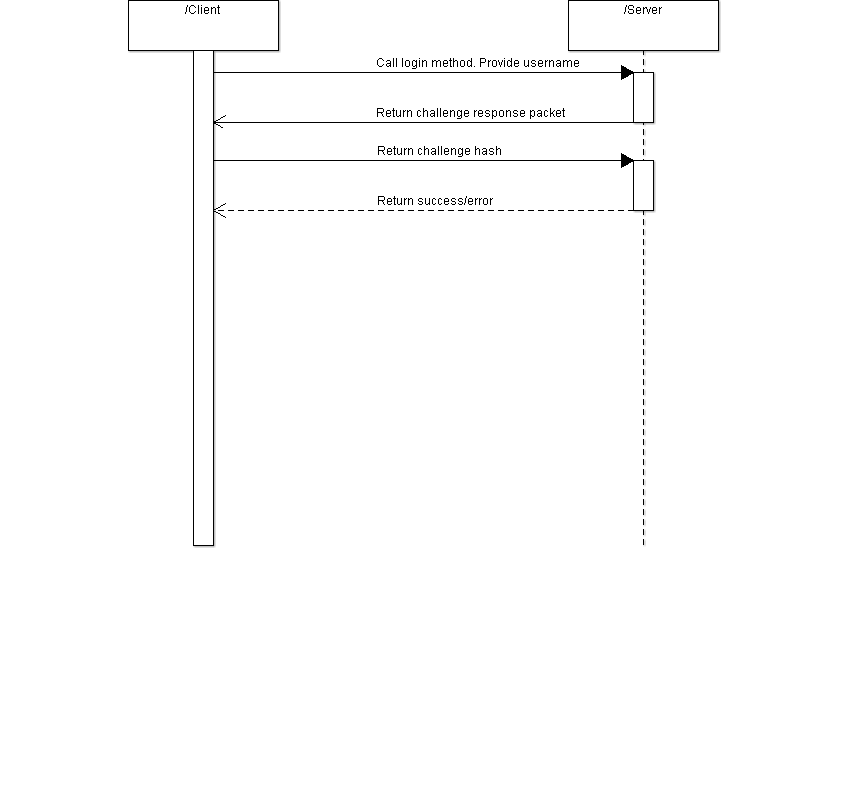
\includegraphics[width=\textwidth]{../images/implementation/embedded_server/SequenceDiagram.png}
	\caption{Client authentification process}
	\label{fig:embedded_server_login_auth}
 \end{figure}
\end{center}




\newpage
\subsection{General purpose client library implementation}
\label{sec:java_library}

\subsubsection{The technology used}
This section will define a client side of embedded service application.
JSON-RPC messages are used as the main application protocol.
Client part should also support all these features that server offers.

\autoref{fig:rpc_call} showed the main architecture of RPC.
RPC client   application usually consists of two modules: client application code
and client RPC stub, that communicates with remote server.
Client calls usual methods on a stub and the code in a stub handles all
the communication magic, it sends requests, receives responses, serialize and
diserialize data objects.

There were already some examples of a small RPC application (see listings
\ref{lst:rpc_server_python_example} and
\ref{lst:rpc_client_python_example})
Our system requirements and environment does not allow to use Python programming
language.
The client application in this work is written for Google Android smartphone
platform, which has a \gls{JVM} virtual machine inside, and the Java programming
language is used.

Java is very popular programming language which is based on \textit{"Write
once, run anywhere"} philosophy. This means a programmer can develop code on a
PC and can expect it to run on any Java enabled hardware, from small embedded systems
to huge server mainframes. 
This is quite mature programming language with lots of libraries and already
written code that solves different problems. For example, see a list Java tools
for JSON at \url{http://www.json.org/}.

The Android system uses Java as one of the main programming language. 
Most programs for android are written using Java and Google provides good
Android development tools for Java programming language.
The Android client application will be covered in the next section, while this one will describe the client
stub library which is written in Java. 
This code can be executed on every hardware that is supported by Java virtual
machines. Application architecture in this projects is based on the ideas of
extensibility and portability and therefore Java is a good choice to start.

I have implemented an universal library for the RPC communication with the
previously described embedded service. That library is easy to add to any Java
project and start to develop a new control application. 
It can be extended to add some required functionality.
 
\subsubsection{Library structure}

The library interface should be identical to a service interface description
or service contract. The JSON service descriptor from the
\autoref{sec:appendix_service_contracts} has enough information to create a
binding library to that embedded service.

This client code can be realized in two different ways: static and dynamic binding.
The library described here, is a static binding library, because it has an already 
defined interface class and client methods are known at the compile time.

Dynamic libraries can determine available server methods at the runtime. Client
library may connect to a server and receives a list of operations. For example JSON
service contract that is used in this work, can be obtained and parsed at the runtime. Dynamic proxy
class can be created from received list of methods and methods can be called
only by a name without the compile time checking. Client may know only a method
name or a part of that name and decide while application is running, which
methods to call. Domain keywords for Java are: \textit{reflection}, \textit{dynamic proxy
class}, \textit{duck typing}. 
The Python example above uses this approach and
you can retrieve list of available methods from server by calling
\texttt{listMethods()} on a \texttt{ServerProxy} object. 
This technique is more suitable for dynamically typed programming languages. 

I preferred to make more robust and simple solution. I created a Java
interface class with all methods that server has. 
The definition of the main interface classes in the library is provided below.

\begin{listing}[H]
\begin{minted}[frame=lines,
               framesep=2mm]{java}
public interface Service {

    // connect methods
    void connect(Reader inputReader, Writer outputWriter);
    boolean isConnected();
    void disconnect();

    public void start();
    public void stop();
    public boolean isRunning();

    boolean addListener(RPCServiceListener listener);
    boolean removeListener(RPCServiceListener listener);

    void setTimeoutMs(long timeoutMs);
    long getTimeoutMs();

    void setRequestProcessor(RequestProcessor requestProcessor);
    RequestProcessor getRequestProcessorByType(
	    Class requestProcessorClass,
	    Object... params);
}               
               
public interface CoffeeMachineService extends Service {
    ServiceContract getServiceContract();
    
    Map<String, Object> getInfo();
    
    // products
    List<Product> getProducts();
    Product.Status orderProduct(int productId);
    Product.Status cancelProduct(int productId);
    Product.Status getProductStatus(int productId);
}
\end{minted}
\caption{RPC client main interface class}
\label{lst:rpc_client_interface_class}
\end{listing}

Some object oriented design techniques are used here to get a more abstract code. 
\texttt{CoffeeMachineService}  extends another
interface \texttt{Service}, which has method that are common to every RPC
service.
\texttt{CoffeeMachineService} interface contains only coffee machine related methods and
inherits other methods from the parent class.

Client can use these classes in the application code and does not need to know
the implementation details. To start using it client needs to create an instance
of \texttt{JsonRpcCoffeeMachineService} ( the implementation of
\texttt{CoffeeMachineService} interface), connect it to \texttt{Reader} and \texttt{Writer} stream objects and after that  user can call RPC methods.

\paragraph{Character encoding} ~\\
Java programming language has the abstraction of \texttt{Reader} and
\texttt{Writer}. These are character stream interfaces that allow to write or
read characters to/from underlying information sources. JSON-RPC is a text
based protocol and we only need to handle character data in our application, but
not binary data.\texttt{Reader} and \texttt{Writer} are parents of
\texttt{InputStreamReader} and \texttt{OutputStreamWriter}, which are bridge
from byte streams to character streams. They transfer bytes to characters and
back using a specified character set\footnote{the mapping between characters and sequences of bytes}.
JVM internally stores characters as 16-bit Unicode variables, but in other
systems character can be:  an US-ASCII seven-bit value, UTF-8 multi-byte
encoding, Extended Binary Coded Decimal Interchange Code (EBCDIC) 8-bit
character encoding and others. Character encoding needs to be specified for
\texttt{InputStreamReader} and \texttt{OutputStreamWriter} in order to convert
data properly. We cannot use byte streams in our library because we cannot
predict in which encoding character data will be received from the data byte
source. It might happen that some byte will have different meaning from what we
expect. Therefore we use an abstraction of \texttt{Reader} and
\texttt{Writer} here.

Client of our library should receive an \texttt{InputStream}  object (operates
with byte streams) from somewhere, provide valid character encoding and create
an \texttt{InputStreamReader} from \texttt{InputStream}, and pass it to
\texttt{connect()} method of the RPC library. The source of an
\texttt{InputStream} may be the array of bytes in the memory, a file on the
disk, a network socket or even String objects. In general words, client should
decide where from data bytes should come, where they need to be written, and
wrap these bytes into character streams.

\paragraph{Message encoding} ~\\

This library assumes that received characters are encoded using
netstrings\footnote{ \texttt{<LENGTH>:<DATA>,} format, for more details see
\autoref{sec:netstrings} } message encoding.
\texttt{MessageReader} class in the library has the implementation of similar finite
state machine parsing algorithm, that was used in the embedded server implementation.
It reads the netstrings encoded messages, extracts the data from them and sends extracted characters to
\texttt{MessageHandler} for processing.


The \texttt{MessageWriter} class composes a valid netstring message and  uses the provided
by a client \texttt{Writer} object to write that message to the destination.
\texttt{MessageWriter} receives JSON  objects,converts them into a String data, wraps them
in a netstring message and sends this character data to the destination.

\paragraph{JSON serialization and the JSON-RPC} ~\\

This JSON-RPC client is based on the \texttt{jsonrpc2-base} library from
Vladimir Dzhuvinov (\url{http://software.dzhuvinov.com}).
This library provides a ready classes for handling JSON-RPC requests and
responses.
\autoref{tbl:jsonrpc2-base_methods} shows the entire lifecycle of a RPC call.



\begin{longtabu} to \linewidth {|p{1cm}|p{1.5cm}|X|p{8cm}|}
 	\caption{jsonrpc2-base library RPC methods \cite{jsonrpc2-base}}
	\label{tbl:jsonrpc2-base_methods} 	 	
\hline 
\multicolumn{1}{|l|}{\textbf{Step}} & 
\multicolumn{1}{l|}{\textbf{Side}} &
\multicolumn{1}{l|}{\textbf{Action}} &  
\multicolumn{1}{l|}{\textbf{Used methods}} \\ 
\hline 
\endfirsthead

\multicolumn{4}{l}%
{{\bfseries \tablename\ \thetable{} -- continued from previous page}} \\
\hline 
\multicolumn{1}{|l|}{\textbf{Step}} & 
\multicolumn{1}{l|}{\textbf{Side}} &
\multicolumn{1}{l|}{\textbf{Action}} &  
\multicolumn{1}{l|}{\textbf{Used methods}} \\ 
\hline 
\endhead

\hline \multicolumn{4}{|r|}{{Continued on next page}} \\ \hline
\endfoot

% \hline \hline
\endlastfoot

		1 &
		Client &
		Create a new request &
		\texttt{JSONRPC2Request()}	
		
		\tabularnewline
		\hline
		2 &
		Client &
		Serialize request to string and send &
		\texttt{JSONRPC2Request.toString()}	
		
		\tabularnewline
		\hline
		3 &
		Server &
		Parse received string back to request object &
		\texttt{JSONRPC2Request.parse()}
		
		\tabularnewline
		\hline
		4 &
		Server &
		Get the request data &
		\texttt{JSONRPC2Request.getMethod()}\newline
		\texttt{JSONRPC2Request.getParamsType()}\newline
		\texttt{JSONRPC2Request.getPositionalParams()}\newline
		\texttt{JSONRPC2Request.getNamedParams()}\newline
		\texttt{JSONRPC2Request.getID()}\newline
		
		\tabularnewline
		\hline
		5 &
		Server &
		Create a response &
		\texttt{JSONRPC2Response()}
		
		\tabularnewline
		\hline
		6 &
		Server &
		Serialise response to string and send back &
		\texttt{JSONRPC2Response.toString()}
		
		\tabularnewline
		\hline
		7 &
		Client &
		Parse received string back to response object &
		\texttt{JSONRPC2Response.parse()}
			
		\tabularnewline
		\hline
		8 &
		Client &
		Check the response for success, get the result/error &
		\texttt{JSONRPC2Response.indicatesSuccess()}\newline
		\texttt{JSONRPC2Response.getResult()}\newline
		\texttt{JSONRPC2Response.getError()}\newline

		
		\tabularnewline
		\hline
	%\end{tabularx} 

\end{longtabu}

\texttt{jsonrpc2-base} is able to serialize Java data types to JSON objects
Listing \ref{lst:jsonrpc2-base_serialization} shows how RPC request object is
created from the standard Java data types and \autoref{tbl:json_java_mapping}
shows how JSON to JAVA mappings are done.

\begin{listing}[H]
\begin{minted}[frame=lines,
               framesep=2mm]{java}
// The remote method to call
String method = "makePayment";

// The required named parameters to pass
Map<String,Object> params = new HashMap<String,Object>();
params.put("recipient", "Penny Adams");
params.put("amount", 175.05);

// The mandatory request ID
String id = "req-001";

// Create a new JSON-RPC 2.0 request
JSONRPC2Request reqOut = new JSONRPC2Request(method, params, id);

// Serialize the request to a JSON-encoded string
String jsonString = reqOut.toString();

// jsonString can now be dispatched to the server...
\end{minted}
\caption{RPC request creating from Java standard data types \cite{jsonrpc2-base}}
\label{lst:jsonrpc2-base_serialization}
\end{listing}


\begin{table}[h]
	\centering	
	\caption{{JSON} \ding{214} {Java} data type mapping in
	\texttt{jsonrpc2-base} library \cite{jsonrpc2-base}}
	\label{tbl:json_java_mapping}
	\begin{tabularx}{0.5\textwidth}{|X|X|}
		\hline
		\textbf{JSON} & \textbf{Java} 	 	\\ \hline	    
		true or false & java.lang.Boolean 	\\ \hline	    
		number & java.lang.Number		 	\\ \hline
	   	string & java.lang.String		 	\\ \hline		
		array & java.util.List		 	\\ \hline
		object & java.util.Map			 	\\ \hline
		null & null		 	\\ \hline			  
	\end{tabularx} 

\end{table}

\paragraph{Data flow} ~\\

This paragraph describes the client stub library RPC call in details. 
Although \texttt{jsonrpc2-base} has classes for handling JSON-RPC message
objects, it does not provide any client functionality. 
We need to write a request handling logic to support the communication with
hardware embedded service.

When client of our library calls any method on \texttt{CoffeeMachineService}
class this method starts to prepare a new request. Service interface
implementation add necessary parameters to RPC request (name, method
parameters, an id), and sends it to request processor.

The whole RPC call process visualized at the \autoref{fig:rpc_call_java} 


\begin{sidewaysfigure}
\centering
\scalebox{0.4}
{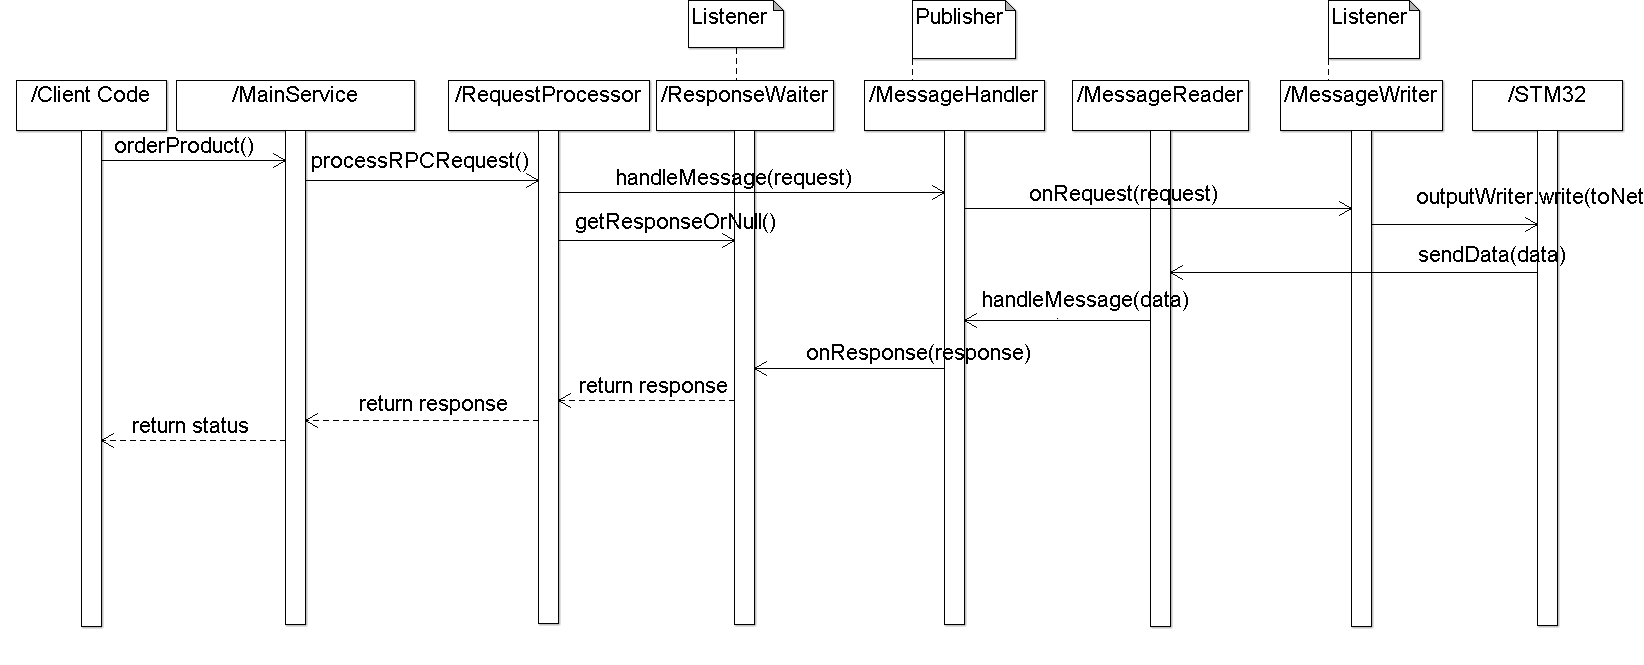
\includegraphics{../images/implementation/java_flow_diagram.png}}
\caption{RPC call in the client stub library}
\label{fig:rpc_call_java}
\end{sidewaysfigure}

\texttt{RequestProcessor} is a simple object with a ~\texttt{Object
processRequest(Object request)} method which encapsulated request processing
logic. Strategy design pattern is implemented here. 
Each request can be processed in a many various ways.
Some methods  have slow execution  on the server and require bigger timeout time
on the client side. Another methods could fail and additional error handling
logic is required. This design methods help to define different  
request handling strategies and apply them at the runtime.
For example the \texttt{getProducts()}  method has very short response time,
because it does not trigger any events on the coffee machine.
Proxy device just returns a list of products from memory storage. 
Another method, the \texttt{orderProduct()}, needs additional communication and
verification of parameters. 
These two methods may have two different algorithms of processing client RPC
request, while programming interface needs to stay fixed.

There is only one strategy for the \texttt{RequestProcessor} implemented yet.
This processor sends a request to a message handler only ones and starts to wait
for a response from a \texttt{RequestWaiter} help class.
After some timeout it returns the result or a \texttt{null} value if there was
not  any response received.

Message writer module of the client stub implements the
\texttt{RPCServiceListener} (pay attention to the 
\texttt{addListener()} and \texttt{removeListener()} methods in listing
\ref{lst:rpc_client_interface_class}) interface. 
This is a \textbf{publish-subscribe mechanism} used in this library for  event
handling.
Service implementation contains a list of service listeners, who are listening
for various RPC messages. 
Listing \ref{lst:event_listener_publisher_interfaces} contains a list o messages that can
be captured by the \texttt{RPCServiceListener}. It also contains a interface of a
class that publishes internal system events.

\begin{listing}[H]
\begin{minted}[frame=lines,
               framesep=2mm]{java}
public interface RPCServiceListener {
    void onRequest(RPCRequest request);
    void onResponse(RPCResponse response);
    void onNotification(RPCNotification notification);
    void onUnknownMessage(String messageText);
}

public interface MessageHandler {
    void handleMessage(String msg);
    void handleMessage(RPCRequest request);
    void handleMessage(RPCNotification notification);
    void handleMessage(RPCResponse response);
}
\end{minted}
\caption{RPC event listener and event publisher interfaces}
\label{lst:event_listener_publisher_interfaces}
\end{listing}

Message writer thread listens for the \texttt{onRequest()} and
\texttt{onNotification()} events. It starts to write request message data to
remote embedded device using the output character \texttt{Writer}  when these
methods are triggered by the request publishers.

System event methods are triggered by a
\texttt{MessageHandler}. This is a small routing class that decides where to put
moving requests, notification, responses and errors according to their types. 
For example, if \texttt{handleMessage(RPCRequest request)} message handler
method is called from somewhere in the code, message handler publishes received
\texttt{RPCRequest} object to all subscribed listeners. 
Message handler calls \texttt{onRequest(RPCRequest request)} method on each
service subscriber and passes new \texttt{RPCRequest} as parameter.

Messages from the the remote device are read by a \texttt{MessageReader} class.
This class reads incoming netstring packets  and passes extracted data
to the \texttt{MessageHandler}. \texttt{MessageHandler} parses incoming JSON 
data and detects that this data type is a JSON-RPC response object. This
Response message becomes published for all listeners including the 
\texttt{ResponeWaiter} help class, who receives message and return it to
\texttt{RequestProcessor}. 


Now the \texttt{RequestProcessor} have received a response it was waiting for
and it can be returned to \texttt{MainService} class. Not the data from the 
response message can be extracted  and remote call result may be returned
to a client code, from where it was initially called.


This is how JSON-RPC messages flow inside service client library.

It might seem quite complicated, but it has lots of advantages. 
Using a publish-subscribe mechanism you might add  multiple event listeners to
the system very easily. 
For example if you need a request logger, you create a class which implements a
\texttt{RPCServiceListener} interface and register it in a main service class 
by calling special methods. Now your logger can listen all RPC
messages and log the information about them.

\paragraph{Conclusion} ~\\

This library can be used in the client application code as the abstract interface of a remote coffee machine.
It makes programming of client code more elegant and easy.
System programmer does not need to develop RPC related code, he can simply use this interface in his projects.
The only necessary step is the connection of a service instance class to the data input and output character streams.
This library uses the netstrings  character data encoding, which is a very simple way how to transfer character data messages.
The whole design is based on the JSON-RPC communication protocol.




%\newpage
\subsection{Implementation of Android client example applications}

The prototype of client-server application was designed during this research project.
The application program was executed on the Google Android operating system powered hardware.


Main idea of this application is the remote wireless control of some electronic device. 
The controlled device example here is a coffee machine, that has some functions like preparing a cup of coffee.
We needed that these functions became available for remote control.

The developed application is a small application with trivial user interface, which allows to prepare products by selecting a product from a small catalogue. 
The screen shot of a ready application is provided  in the \autoref{fig:android_app_screen}

\begin{center}
 \begin{figure}[h]
	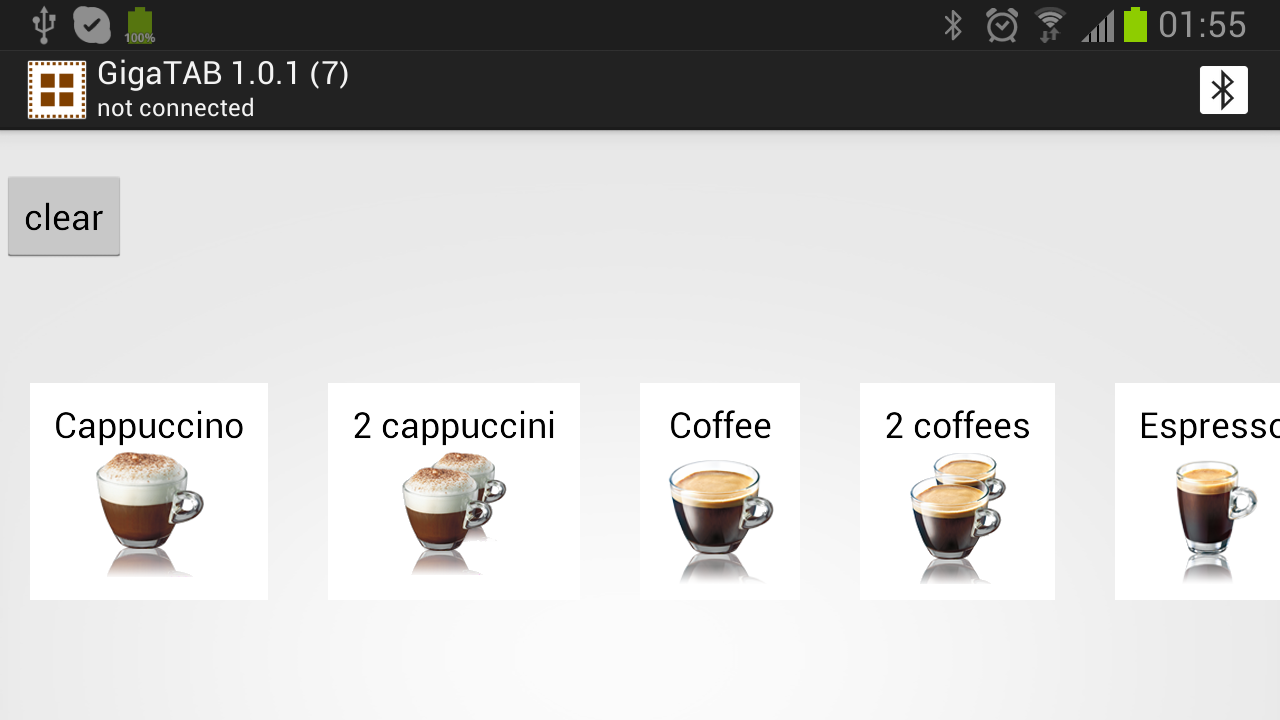
\includegraphics[width=\textwidth]{../images/implementation/android_app_screen.png}
	\caption{Android application visual interface }
	\label{fig:android_app_screen}
 \end{figure}
\end{center}

The usage scenario starts from the connection to coffee machine.
There is a small button with Bluetooth icon in the top right corner of the application.
This button activates a device select dialog, where you can find a remote device by name and MAC address and connect by selecting it in the list.
When connection is established some available products become showed in the horizontal list layout.
It is able to point to each of these products and open a dialog box with detailed information about each product.
User can start coffee preparing from that dialog.
While operation is in progress, it is still possible to cancel the product preparing operation.

I will not cover in details the whole process of the user interface and application creation.
This is out of the scope of this research work and it requires some additional domain knowledge. 
You need to get familiar with Google Android development tools,
read a documentation course, follow the tutorials and study by doing.
There are available lots of application examples and it is not very hard to produce a similar application.
This application is partially based on the Bluetooth chat communication example from the Android Software development kit.

Whole communication is performed over wireless Bluetooth protocol.
It is assumed, that Bluetooth is the abstract transport that can send data bytes over radio link.
The Android Bluetooth API functions can search to nearby Bluetooth devices and provide you a list of \texttt{BluetoothDevice} objects.
You can find your wireless device in that list and tell the Android OS to connect to that device. 
This device list is also used to fill a device choosing graphical dialog described before.

When devices get connected  it is able to receive a communication socket object and get a standard \texttt{java.io.InputStream} and \texttt{java.io.OutputStream} from that.
This is a final step of establishing the communication and it is able to transfer data over received stream objects.


The client RPC library is connected to these streams and it is able to communicate with a remote device over the wireless serial interface.
RPC calls may be started right after application gets connected to the Bluetooth input and output streams.


Now it is up to your imagination how to use and extend this remote embedded service.
You can implement any rich functionality and create whatever complex system you want or your hardware resources allow you.
This extensible service oriented embedded architecture allows you to do so.

	
	%\newpage
\section{Conclusions}

Several possible variants of SOA implementation were covered in this work.
Some of them are mature and standardized tools which are used in many production
systems nowadays.
Another ones are lightweight and beautiful alternatives to the first group. They
can be  used even in the small microcontroller devices. 
Their specifications does not tie a programmer to work with a limited specific
set of technologies. 
Some of covered tools can be used in any environment and support all creativity
of the developers. 
JSON and XML, the ideas of RPC, they all can be used in many various ways.

Author was trying to analyse all of them in his research.
This work chosen some comparison of SOA implementations and related technologies
is the context of the embedded systems.
Some technologies were chosen for the trial.
The choice of the technologies  does not mean that they are the best and the
only suitable solution for the application described here.
Author's  aim was to show that it is possible to create the systems of small
devices using lightweight protocols and data structures.

Some specific application field was chosen as an example in this work.
Lets watch how it was realized and overview the results.

\subsection{Results}

There was a defined goal of this work: make a research of available
machine-to-machine communication techniques and deliver a functional system
prototype to fulfill some business needs.

Author has a freedom of choosing any suitable technology and was limited only
with the available hardware platform. 
This work can be characterize as a research activity of detecting possible
facilities, not than an implementation of specific task of interconnecting
a mobile phone and the coffee machine.
There should be a goal to reach, some problem which needs a solution in order to
start watching around. 
I have defined this abstract task and decided to make a
case study about it.

One of multiple ways how to design a client-server system is the
SOA. Services are self-describing and open components, which use standard
communication schemes. 
Author of this work was inspired by this approach and have created a SOA
based system.


This paper contains a research of different technologies that help to implement
services on the devices.
It is unable to find and analyse all possible solutions. The most popular and
open approaches were analysed instead. 
Author has chosen a concept of remote procedure calls and found a simple
and lightweight solution of JSON-RPC. 

I had no experience of programming microcontrollers before. The company, where i
was doing my university internship, provided me one specific microcontroller
family and my task was to learn how it can be applied. To find out the
hardware possibilities you need to study the  architecture of a specific
devices.
This work became for me not only a research project, but  a complete
microcontroller practical course.
I have learned how to use different development tools and STM32F1 and other ARM
Cortex-M3 microcontroller hardware platform features, exercised low level C
programming and even soldered wires on development boards to repair boundary
scan debugger.
This was done only by myself with the help of internet resources
and other information sources.
This was the largest laboratory work i have ever experienced.

A small remote service was finally implemented on a STM32F103ZE microcontroller. 
This server is able to response for remote client requests and provide some
useful services.
This device is a proxy bridge between client application and coffee machine
hardware.
Only a few set of functions were implemented, but this functionality reflects all
the architecture features.
It is able to determine the structure of this system by tracing how a
single RPC request is transferred between different system modules..

This solution uses embedded realtime operating system FreeRTOS, so i was
involved in a development of a parallel and multitasking system. 
Server program consists of parallel tasks, which are communicating to each other
and process incoming requests. Internals are implemented as chain of
processing units, which pass work to each other.

The client side of application is designed as a Java library that can be used
in any kind of client application. It provides remote device methods and handles
all communication between the client code and embedded service server.

This library  is used inside the Android demo application, that is executed on
the mobile phone or tablet.
Android program was designed to be an example application case. 
This provides some controls over the remote coffee machine. 


The goal of this work was achieved.
This was a research of a big bunch of technologies: embedded hardware related
highly constrained and optimized software was studied together with  modern
internet technologies that connect billions different machines.

Lots of new things and interesting computer science approaches were found during 
accomplishing the tasks and information mining.
Obtained experience and knowledge would help me to
deliver more quality products in future and not to make those mistakes that
every young computer system engineer does.

\subsection{Future work}
This small implementation of client-server application connects together only
two devices. 
This does not define any additional methods how to find
devices in a network and connect other devices.
This is only an abstract service architecture that was designed to be universal.

There is no security, addressing, discovery and quality of service. 
It requires some reliable transport protocol stack that covers data transferring
from physical communication layer up to application layer.

In order to become a real world product and be integrated to other systems 
there should be dedicated connectivity requirements.
Devices should be connected in some standard way. 

Most of reviewed information sources covered the development of embedded services in
context of internet and TCP/IP networks.

I see the next development cycle of this architecture to be the integration to
the Internet of Things.
Many research groups are working on developing distributed communication for
small embedded devices and wireless sensor networks on the Internet. 
Their work papers include keywords like 6LoWPAN, IEEE 802.15.4, IPv6, RPL,  UDP, COAP, RESTful embedded services.

\autoref{fig:future_technologies} shows how this technologies could be applied.

\begin{figure}[H]
        \centering		  
		  \begin{tabular}{c}
			\subfloat[Optimized IP protocols]{
				\label{fig:optimized_ip_stack}
				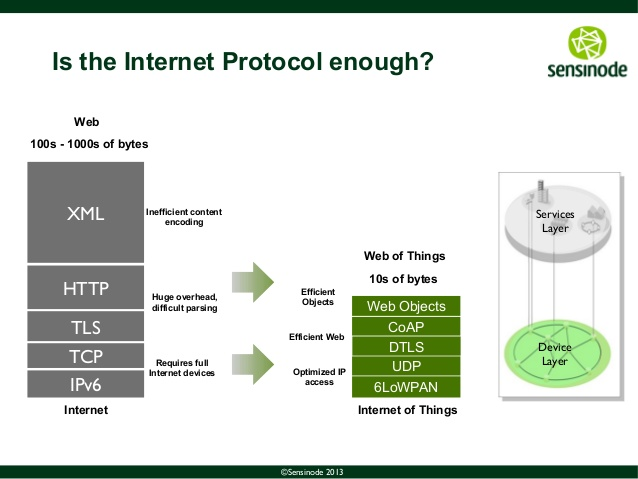
\includegraphics[width=0.5\textwidth]{../images/optimized_ip.jpg}
			} \\
			\subfloat[RESTful Web things Things architecture]{
				\label{fig:restful_wot}
				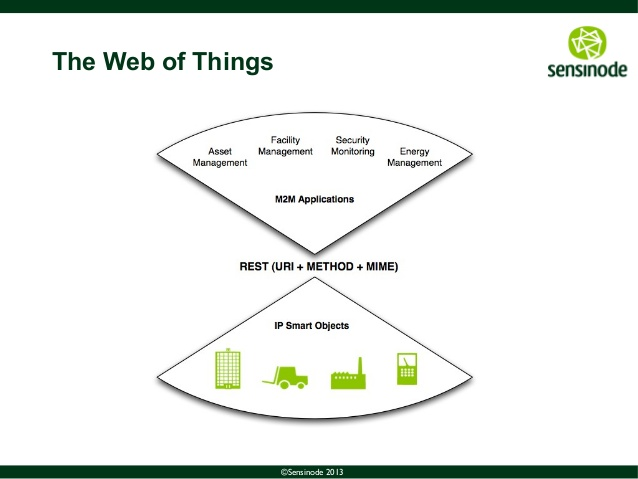
\includegraphics[width=0.5\textwidth]{../images/restful_WoT.jpg}
			} \\
			\subfloat[RESTful temperature sensor usage example]{
				\label{fig:restful_sensor}
				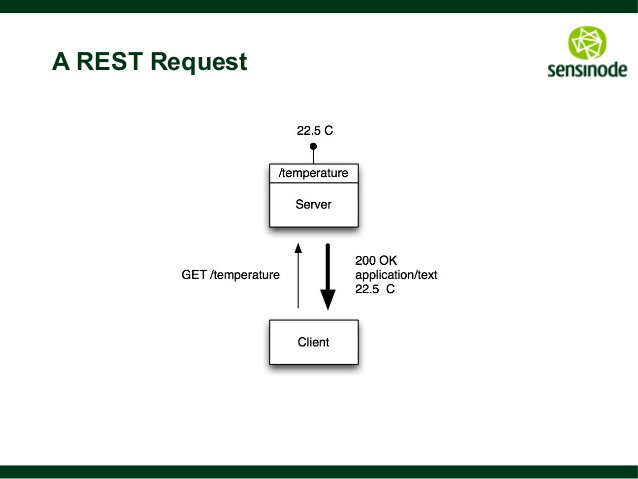
\includegraphics[width=0.5\textwidth]{../images/restful_temperature_sensor.jpg}
			} 
		  \end{tabular}        
        \caption{Optimized internet technologies for networked embedded systems~\cite{iot_standards,CoAP_Tutorial}}
        \label{fig:future_technologies}
\end{figure}


During this research i have found a project named Contiki.
Contiki is an open source operating system for networked, memory-constrained systems with a particular focus on low-power wireless Internet of Things devices.
Examples of where Contiki is used include street lighting systems, sound monitoring for smart cities, radiation monitoring systems, and alarm systems.\footnote{\url{http://www.contiki-os.org/}}

This project supports  very resource efficient  full IP networking\footnote{ uIP TCP/IP Stack from Adam Dunkels. See ~\cite{Dunkels07programmingmemory-constrained} } and is optimized for tiny systems, having only a few kilobytes of memory available. 
This is a good candidate to be the main technology of this kind of system we have been developed here.

Our design could be rewritten for the Contiki OS and we could migrate to the hardware used in wireless sensor networks.
This could be a very tiny chip with some wireless interface onboard.
It is able to build very low-power and low-cost embedded web service  using this technology stack.

This kind of work requires another exhaustive research and laboratory experiments.
This field is the topic of interest of many scientists and companies, who produce networked embedded solutions.
It is quite popular nowadays and there are many use cases and benefits using distributed embedded network computing.

More and more devices gets connected to the internet. 
This technologies could help to improve the quality of our lives by
introducing a network of low-cost and low-power sensors and actuators. 



	
	\section{Examples of service contracts}
\label{sec:appendix_service_contracts}

Example of WSDL contract from WSDL documentation~\cite{wsdl_language_spec}:
%\begin{listing}[H]
\inputminted[linenos=true,tabsize=4,fontsize=\footnotesize]{xml}{../source/service_contract/wsdl_example.xml}
\label{lst:wsdl_example}

%\begin{landscape}
%\large{TODO put last version of contract here}
Example of JSON service descriptor:
%\begin{listing}[H]
\inputminted[linenos=true,tabsize=4,fontsize=\footnotesize]{json}{../source/service_contract/service_schema.json}
\label{lst:json_contract_example}

%\end{landscape}
%	\caption{Example of WSDL contract from WSDL documentation.}
	
%\end{listing}


	
	\newpage
	\listoffigures
	\newpage
	\listoftables
	
	
	\bibliographystyle{ieeetr}
	\bibliography{../resource/references}
	

\end{document}